%
% erklaerung.tex
%
% (c) 2019 Prof Dr Andreas Müller, Hochschule Rapperswil
%

\documentclass[10pt]{standalone}
\usepackage[utf8]{inputenc}
\usepackage[T1]{fontenc}
\usepackage{cancel}
\usepackage{times}
\usepackage{amsmath}
\usepackage[english,ngerman]{babel}
\usepackage{amssymb}
\usepackage{amsfonts}
\usepackage{amsthm}
\usepackage{fancyhdr}
\usepackage{graphicx}
\usepackage{txfonts}
\usepackage{tikz}
\usetikzlibrary{shapes.geometric,arrows,automata,calc}
\begin{document}
\sffamily
\begin{tikzpicture}[>=latex]

\fill[color=white] (-6.5,-5.5) rectangle (10.2,5.5);

\node[opacity=1.0] at (0,0) [right] {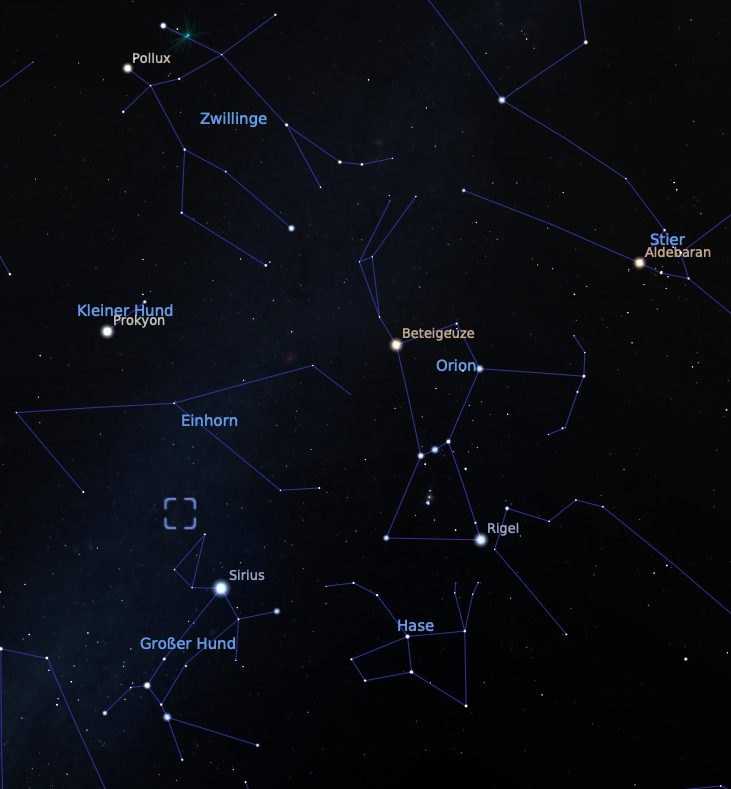
\includegraphics[width=10cm]{sternkarte.png}};

\node at (-6,4.5) [right] {\Large Seemöven-Nebel};

\node at (-6,0.0) [right] {\begin{minipage}{5.4cm}
\sffamily
\raggedright
Der Seemöven-Nebel IC2177 ist ein
3650 Lichtjahre entfernter Emissionsnebel.
Interstellares atomares Wasserstoffgas wird von einem hellen Stern
ionisiert und zum Leuchten in der roten H-$\alpha$ Spektrallinie
angeregt.
\medskip

IC2177 wurde im 19.~Jahrhundert vom walisischen
Amateur- Astronomen und Astrophotographie- Pionier Isaac Roberts entdeckt. Er
befindet sich im Grenzgebiet zwischen den Sternbildern Einhorn und grosser
Hund, ungefähr auf einem Drittel der Distanz zwischen den hellen Sternen
Sirius und Prokyon.

\end{minipage}};

\draw[color=white] (-6.5,-5.5) rectangle (10.2,5.5);

\end{tikzpicture}

\end{document}



